
%place your content here, feel free to create subcontent files


\begin{block}{\blocktitle{Synthetic Single-Task Benchmark}}
\begin{itemize}
 \item Target functions sampled from a generative model (GP with isotropic RBF kernel
of length scale $l = 0.1$ and unit signal variance) on $\mathcal{X} = [0, 1]^2$ 
 \item In practice: sample $250$ function values from GP, fit GP to these function values and use resulting posterior mean as target function
 \item Gaussian noise with standard deviation $\sigma =10^{-3}$ is added to each observation
 \item Model mismatch: target functions from GP with rational quadratic kernel but RBF kernel in surrogate model
\end{itemize}

\begin{center}

\begin{figure}
\centering
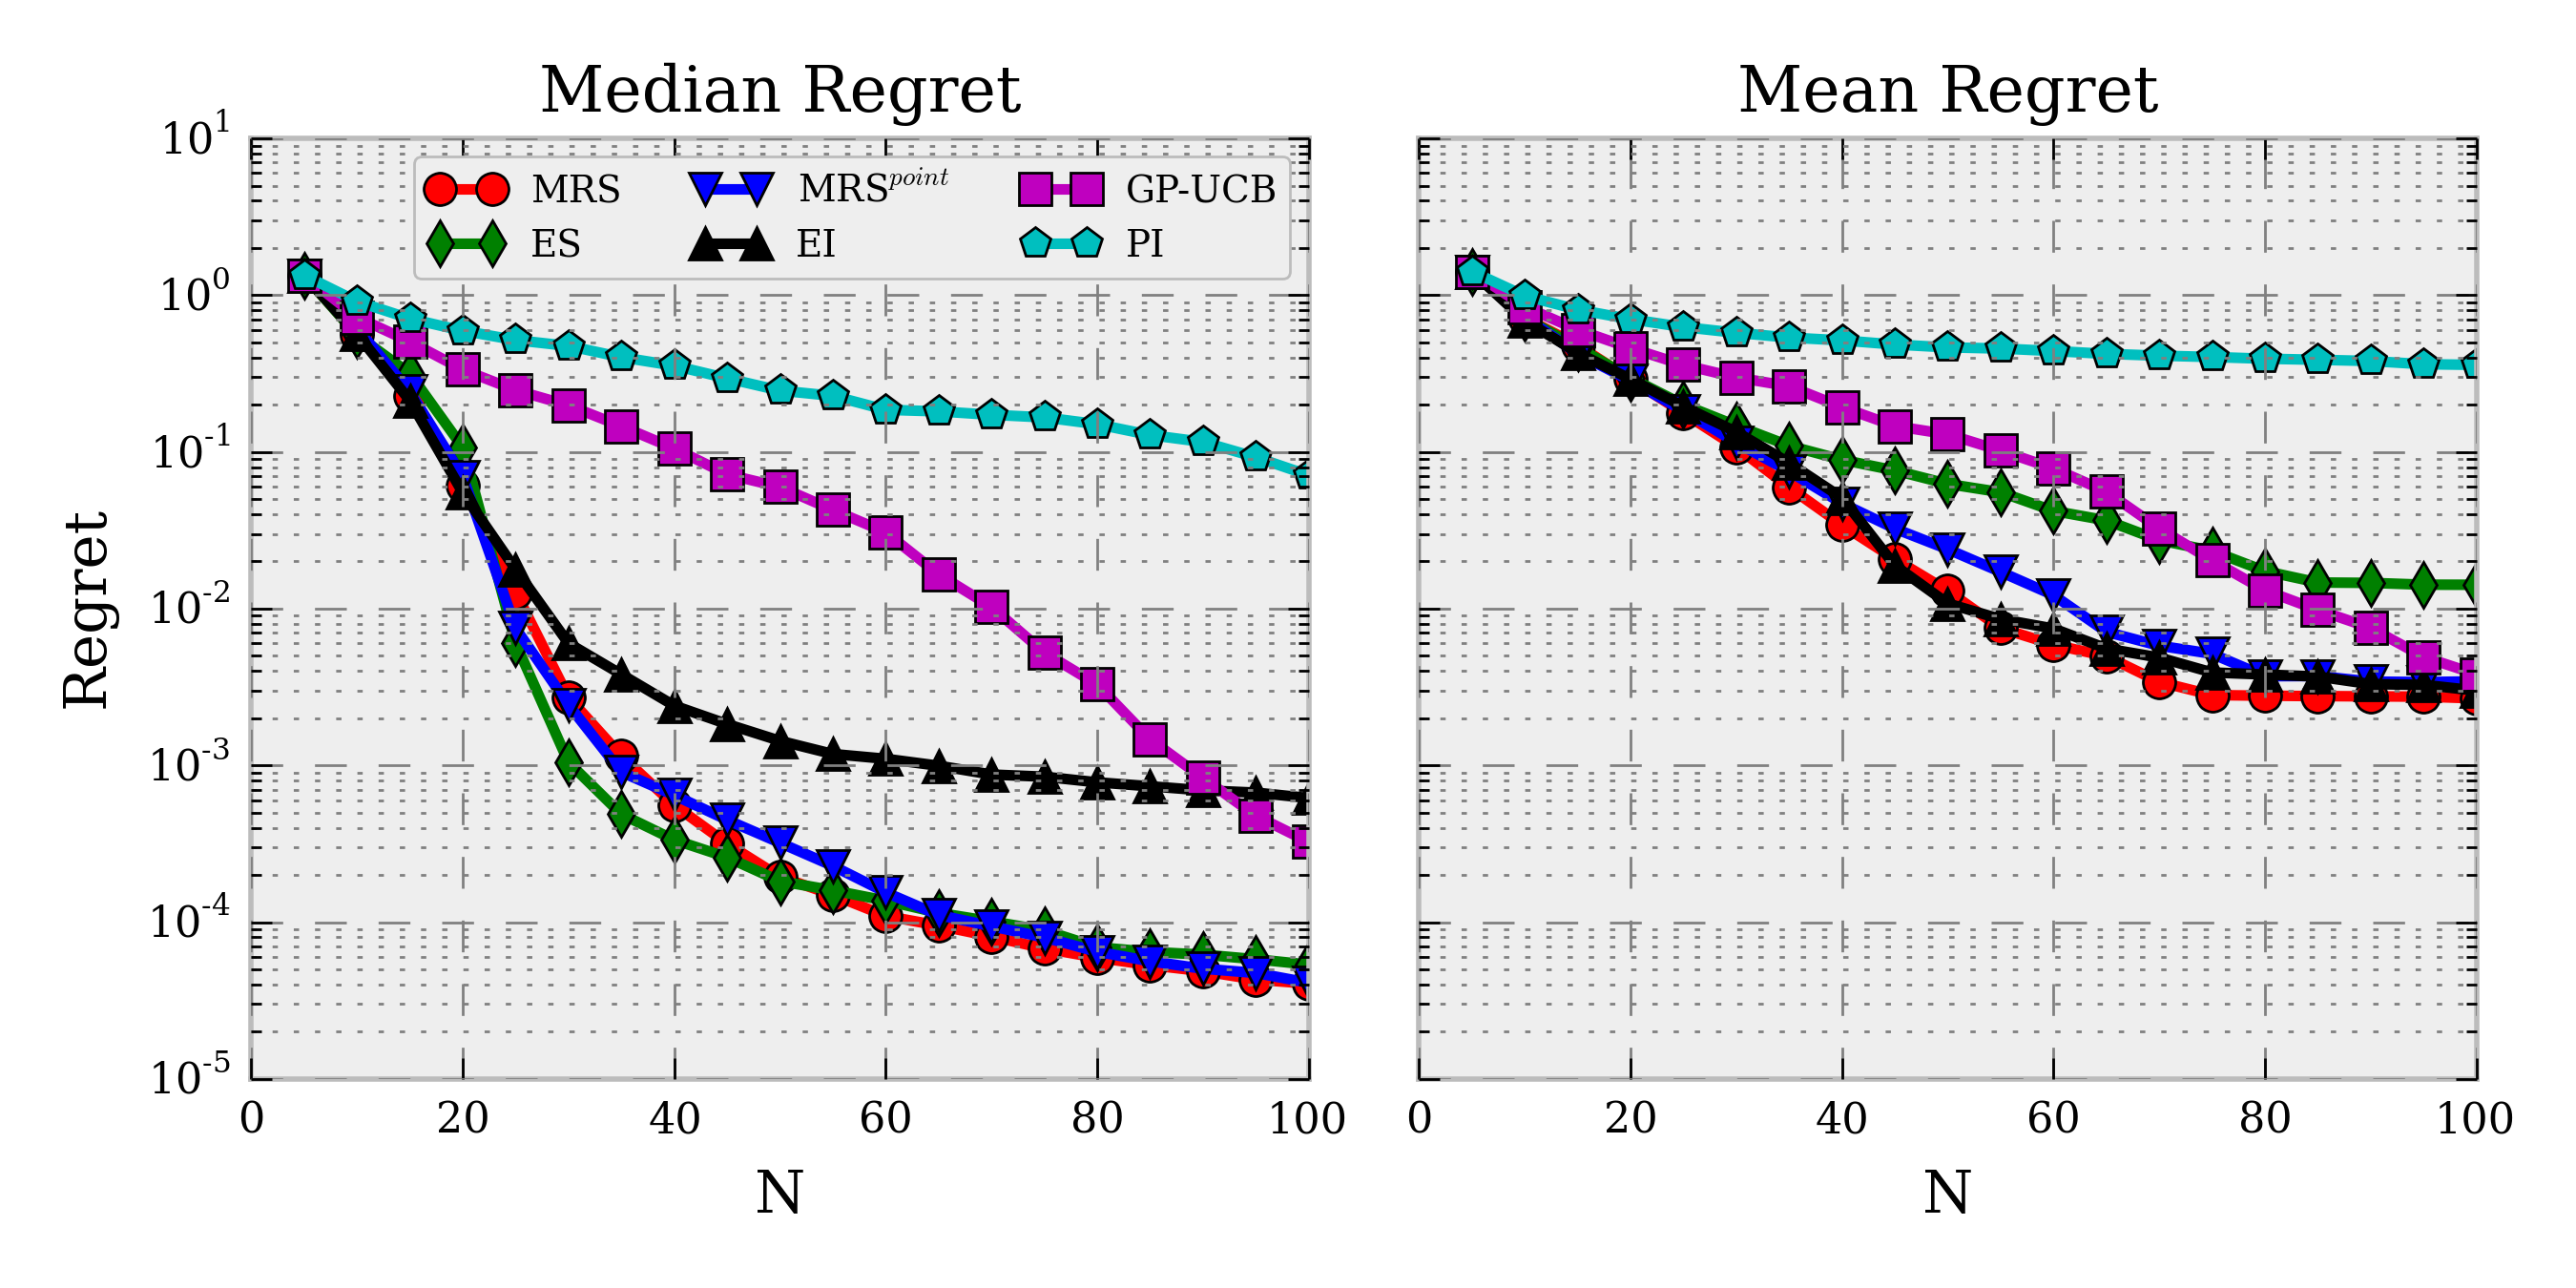
\includegraphics[width=.8\columnwidth]{../pics/empirical_comparison} \\
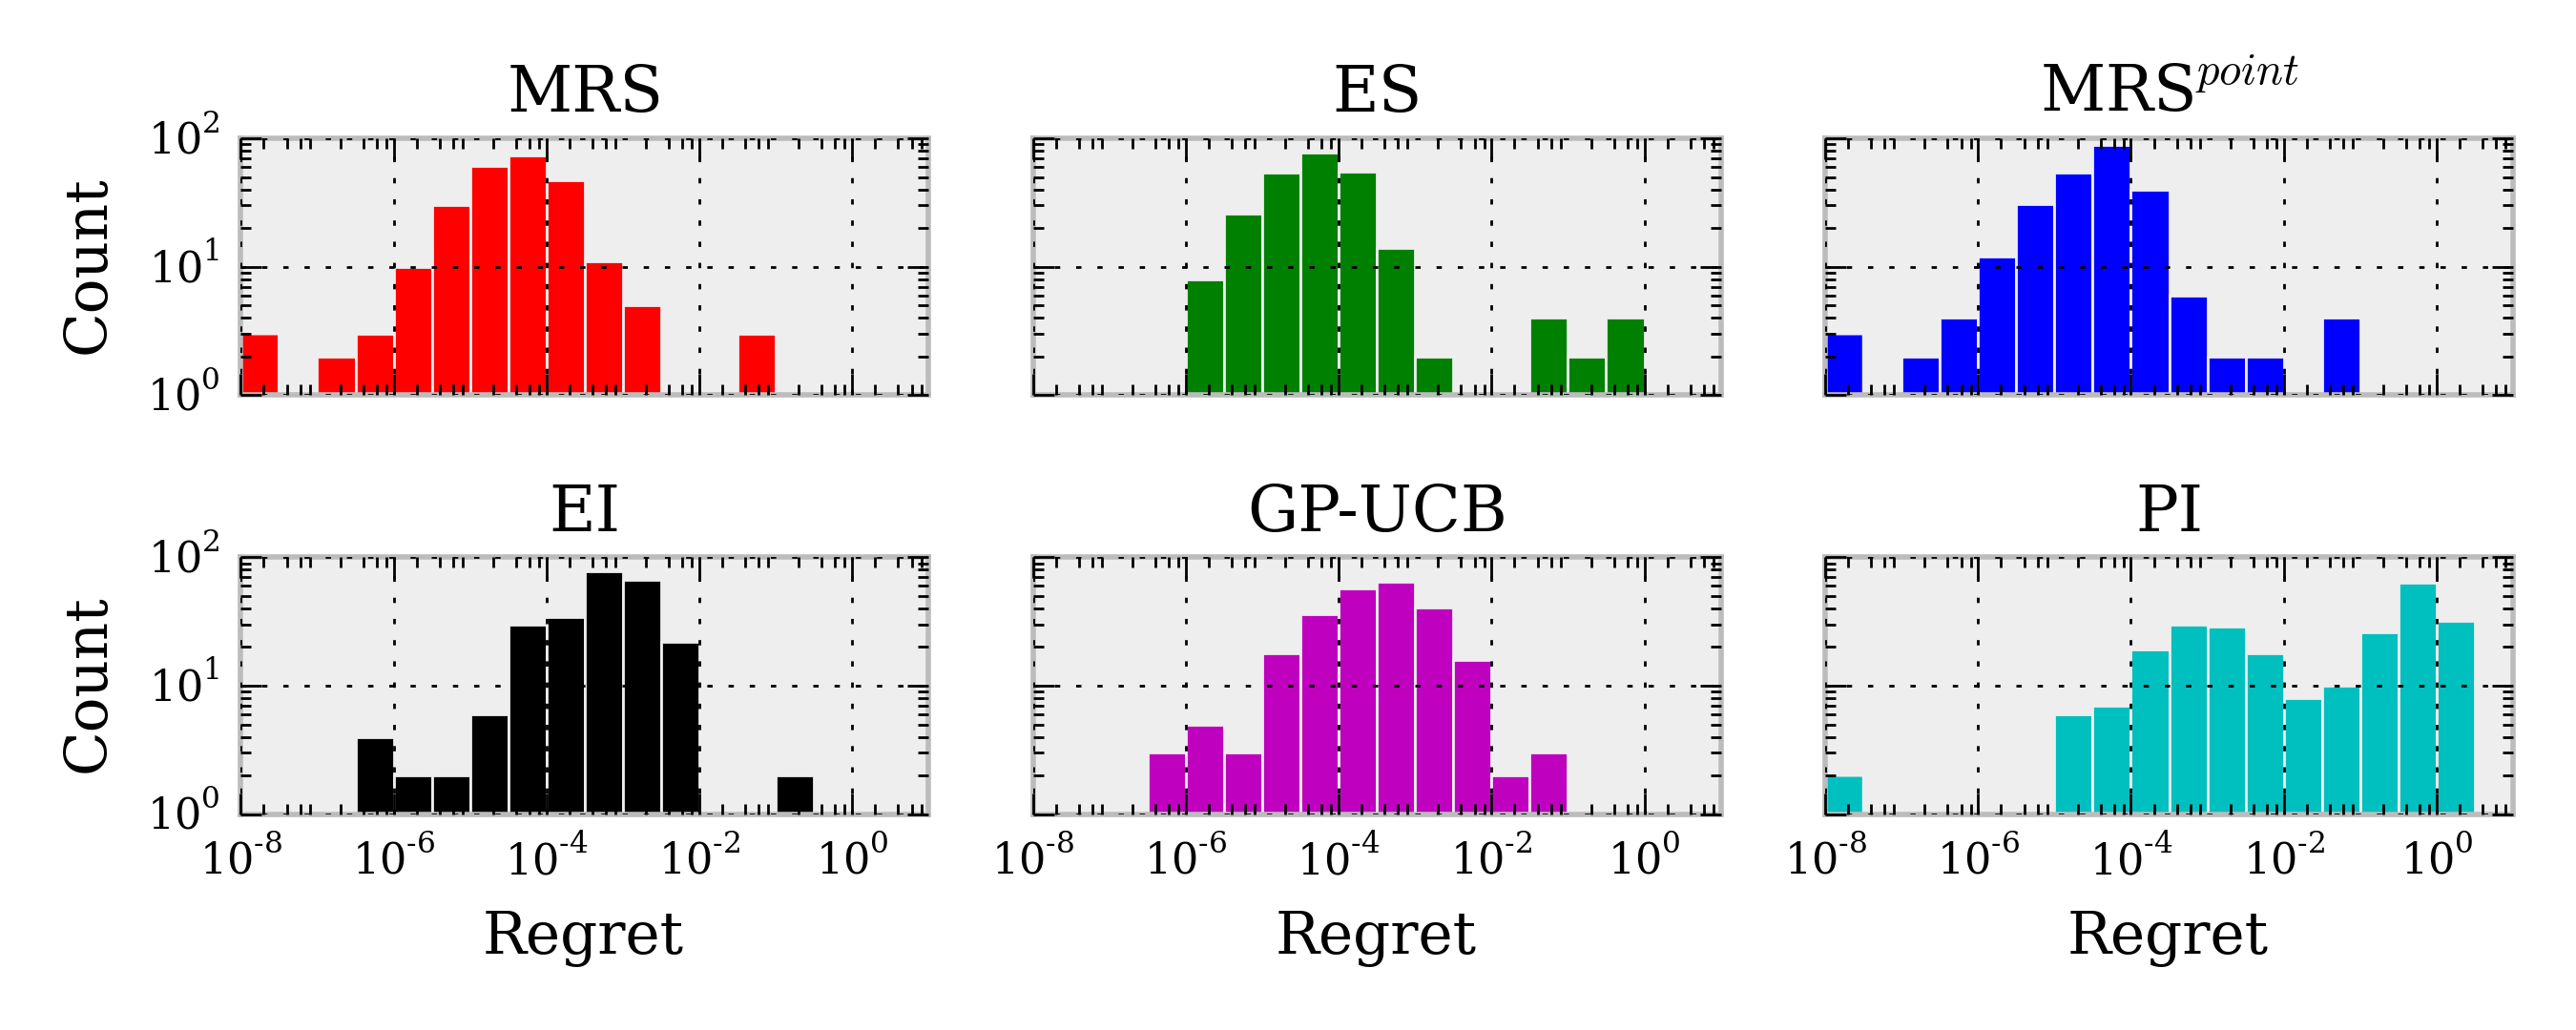
\includegraphics[width=.8\columnwidth]{../pics/hist}
\caption{Simple regret of the recommendation $\mathbf{\tilde x}_N$ after $N$ trials over $250$ repetitions for different acquisition functions (\emph{no model mismatch})}
\label{fig:empirical_comparison}
\end{figure}


\begin{figure}
\centering
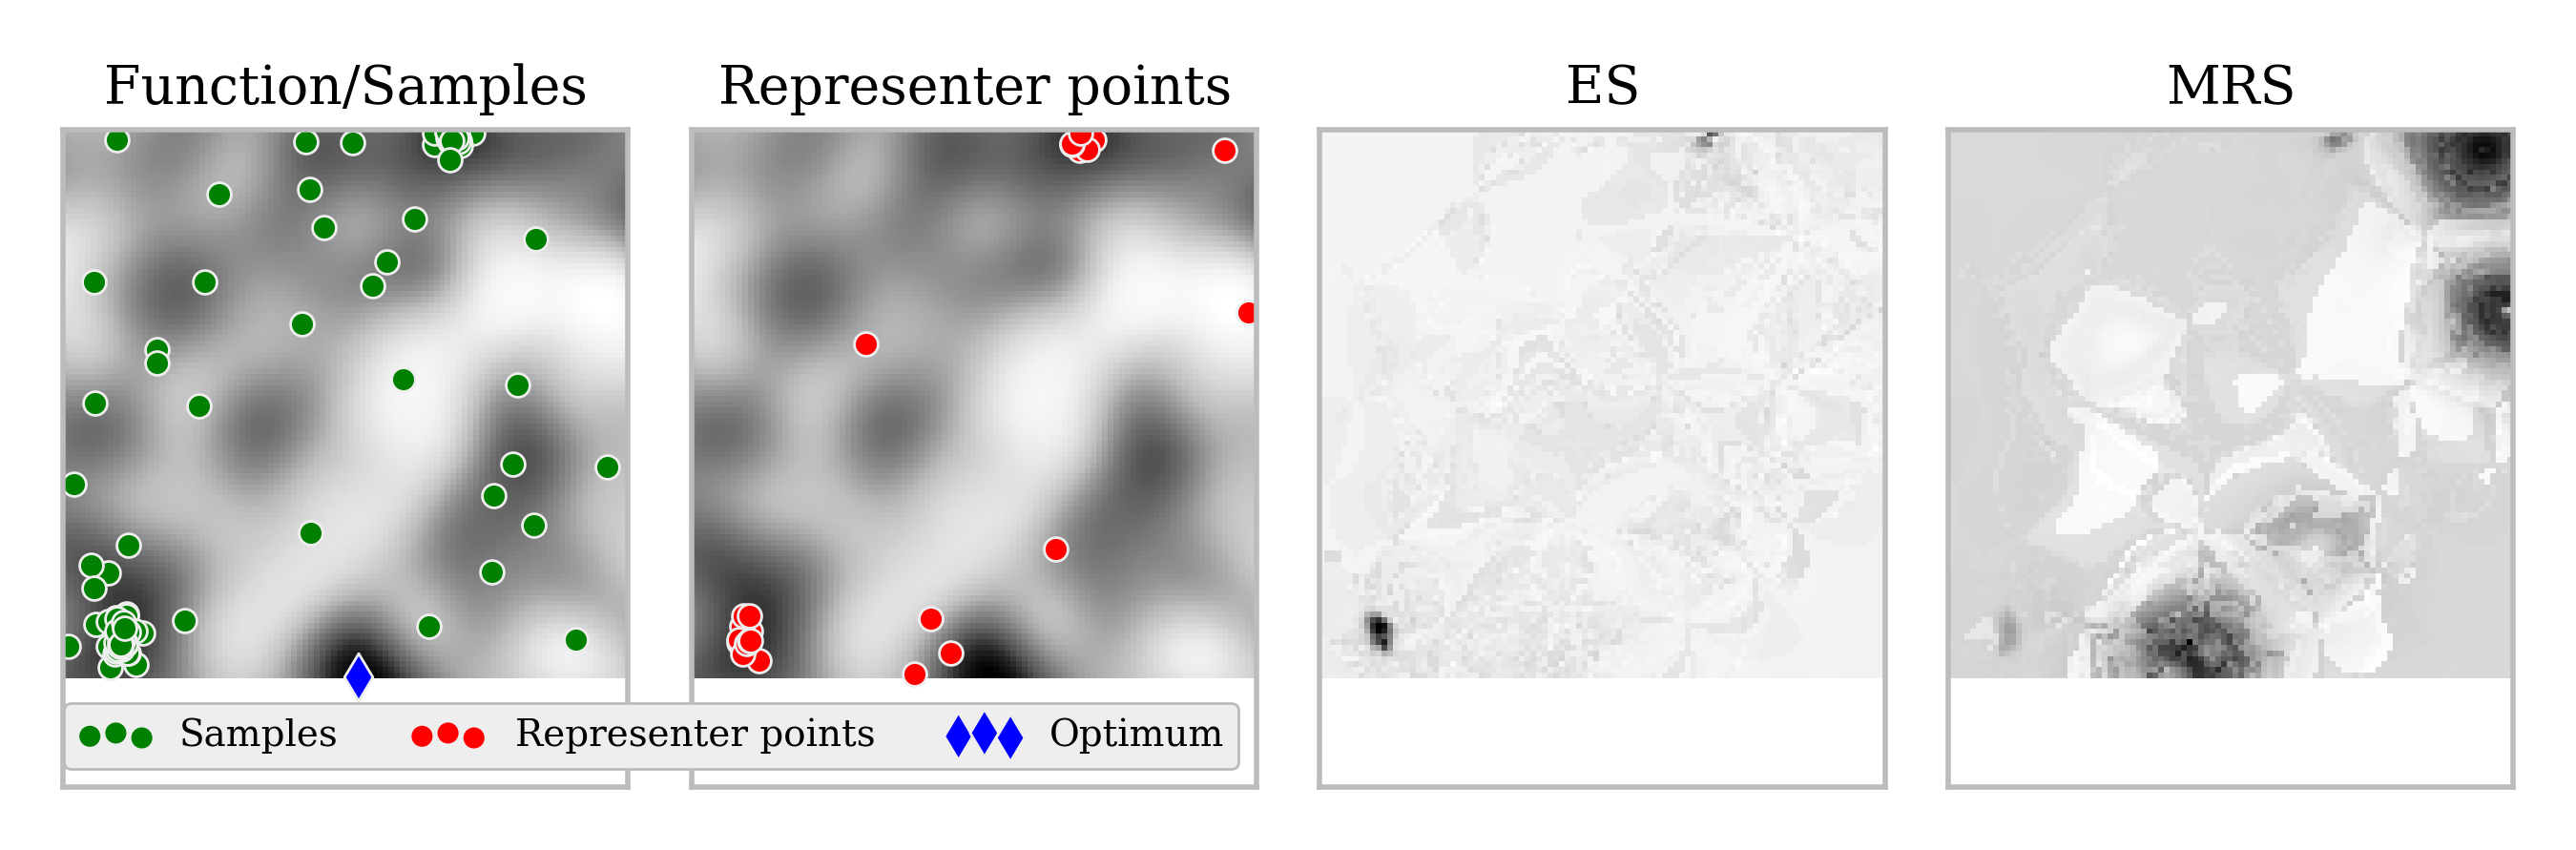
\includegraphics[width=.8\textwidth]{../pics/es_analysis}
\caption{Acquisition functions on a target function at $N=100$ and 25 representer points; darker areas correspond to larger values. ES focuses on sampling in areas with high density of $p^\star$ (many representer points), while MRS focuses on unexplored areas that are populated by representer points (non-zero $p^\star$).
}
\label{fig:es_analysis}
\end{figure}


\begin{figure}
\centering
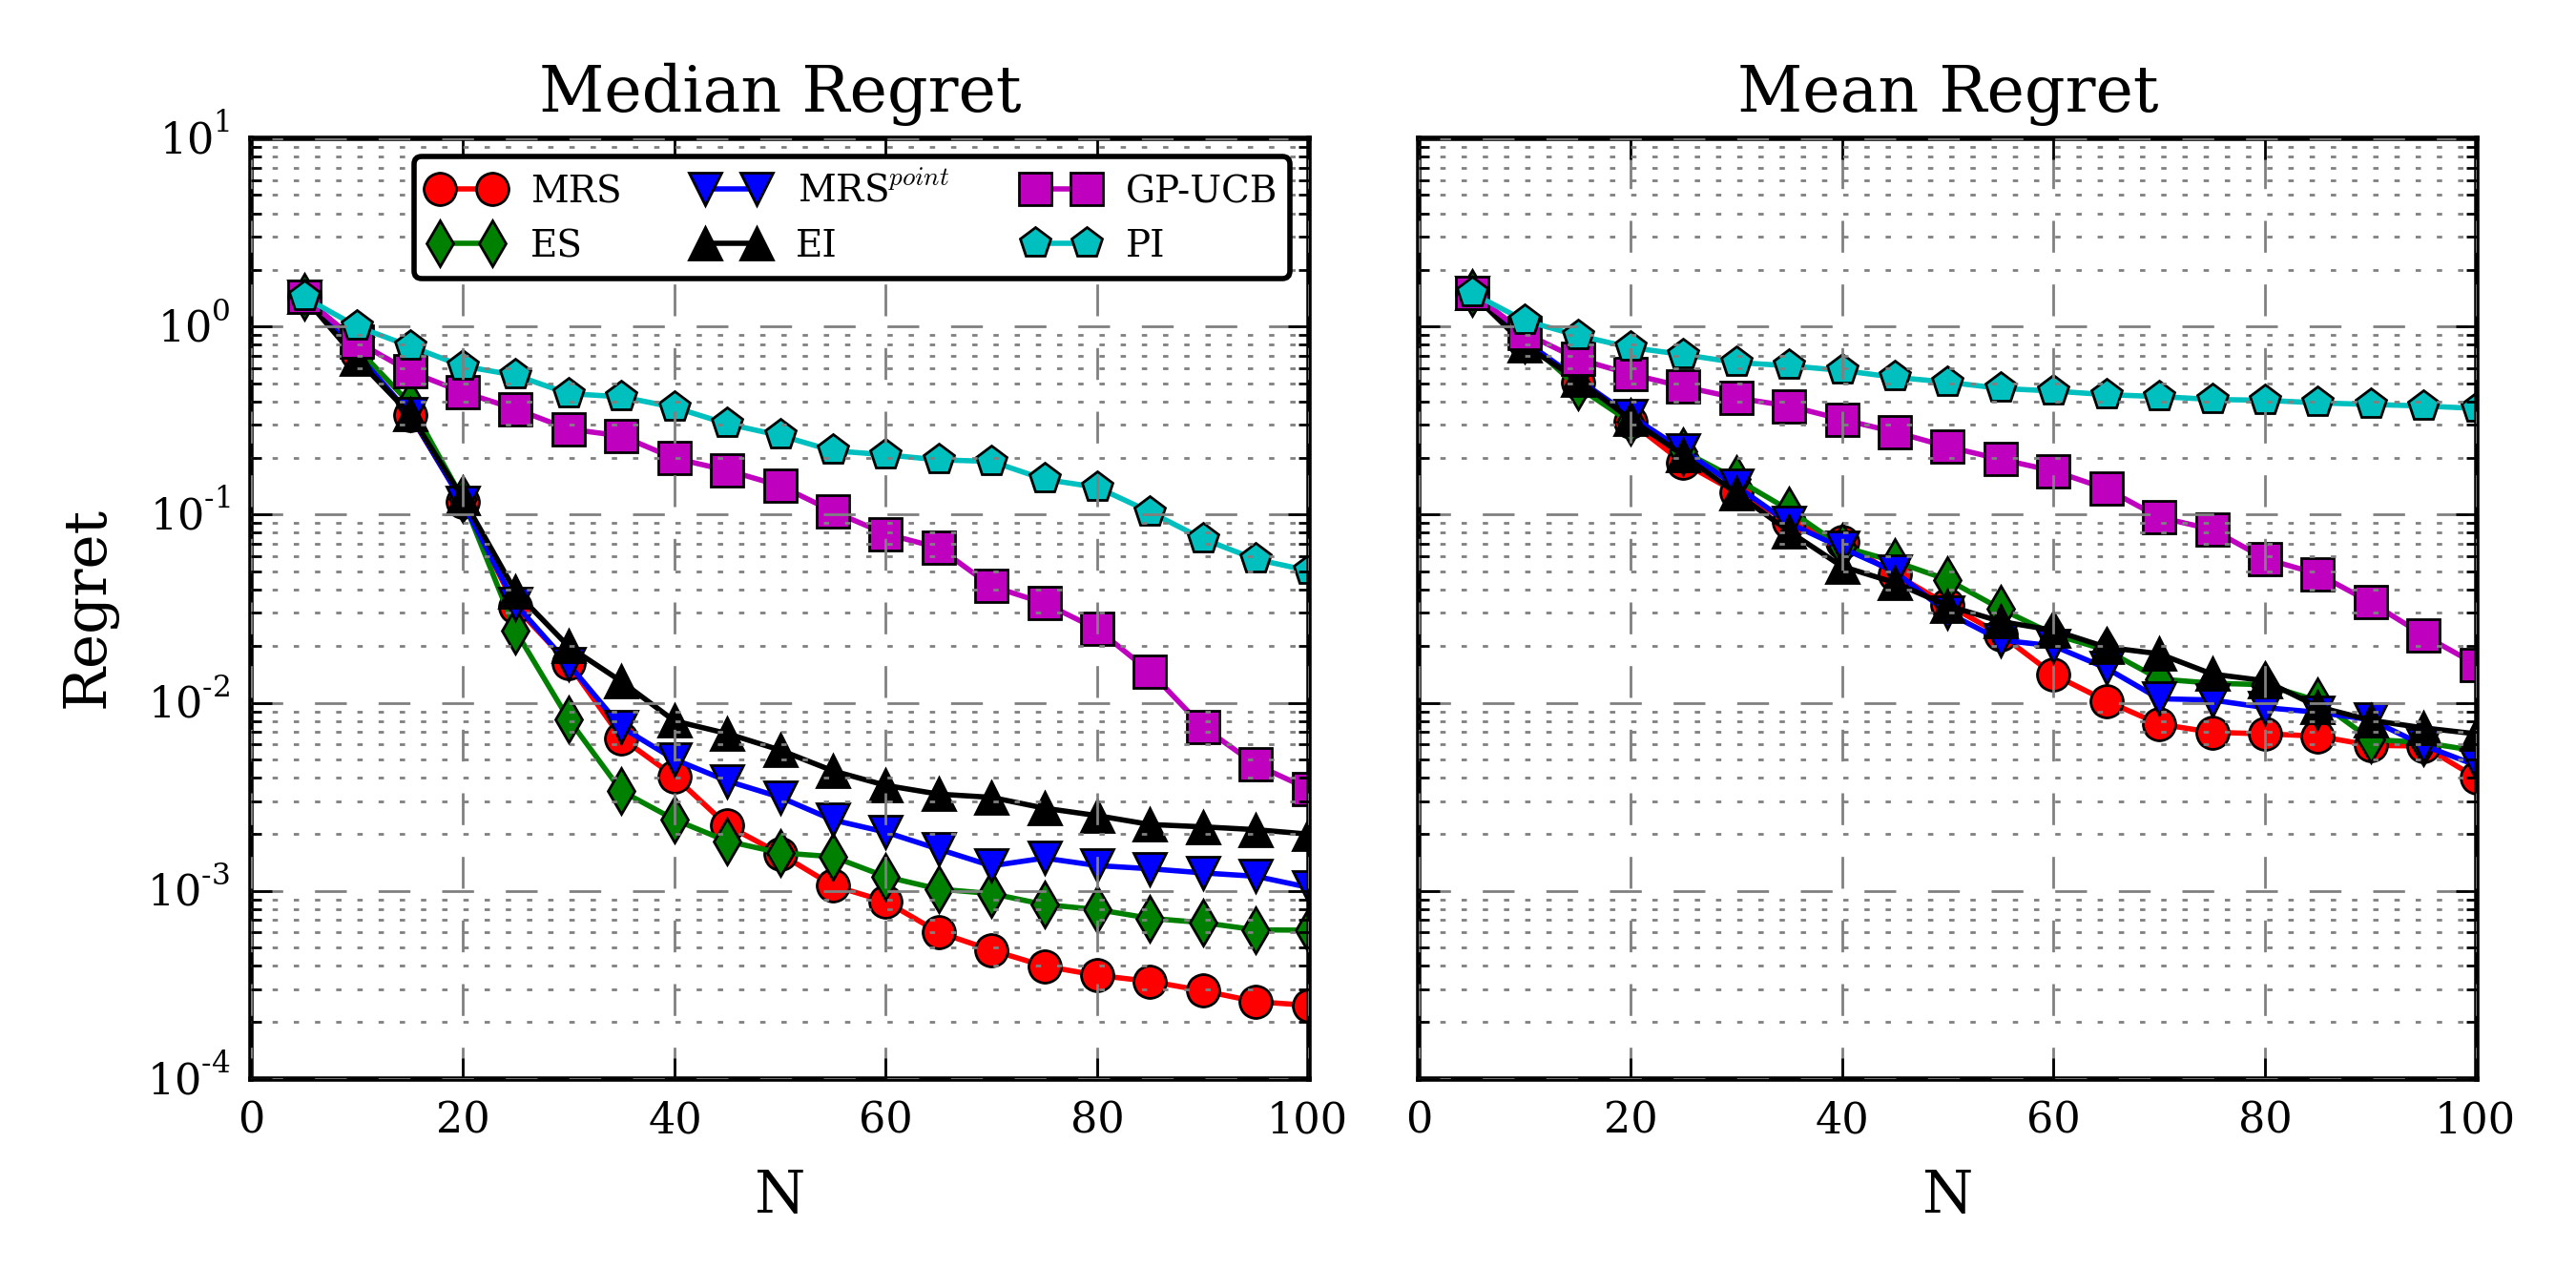
\includegraphics[width=.8\textwidth]{../pics/empirical_comparison_mm} \\
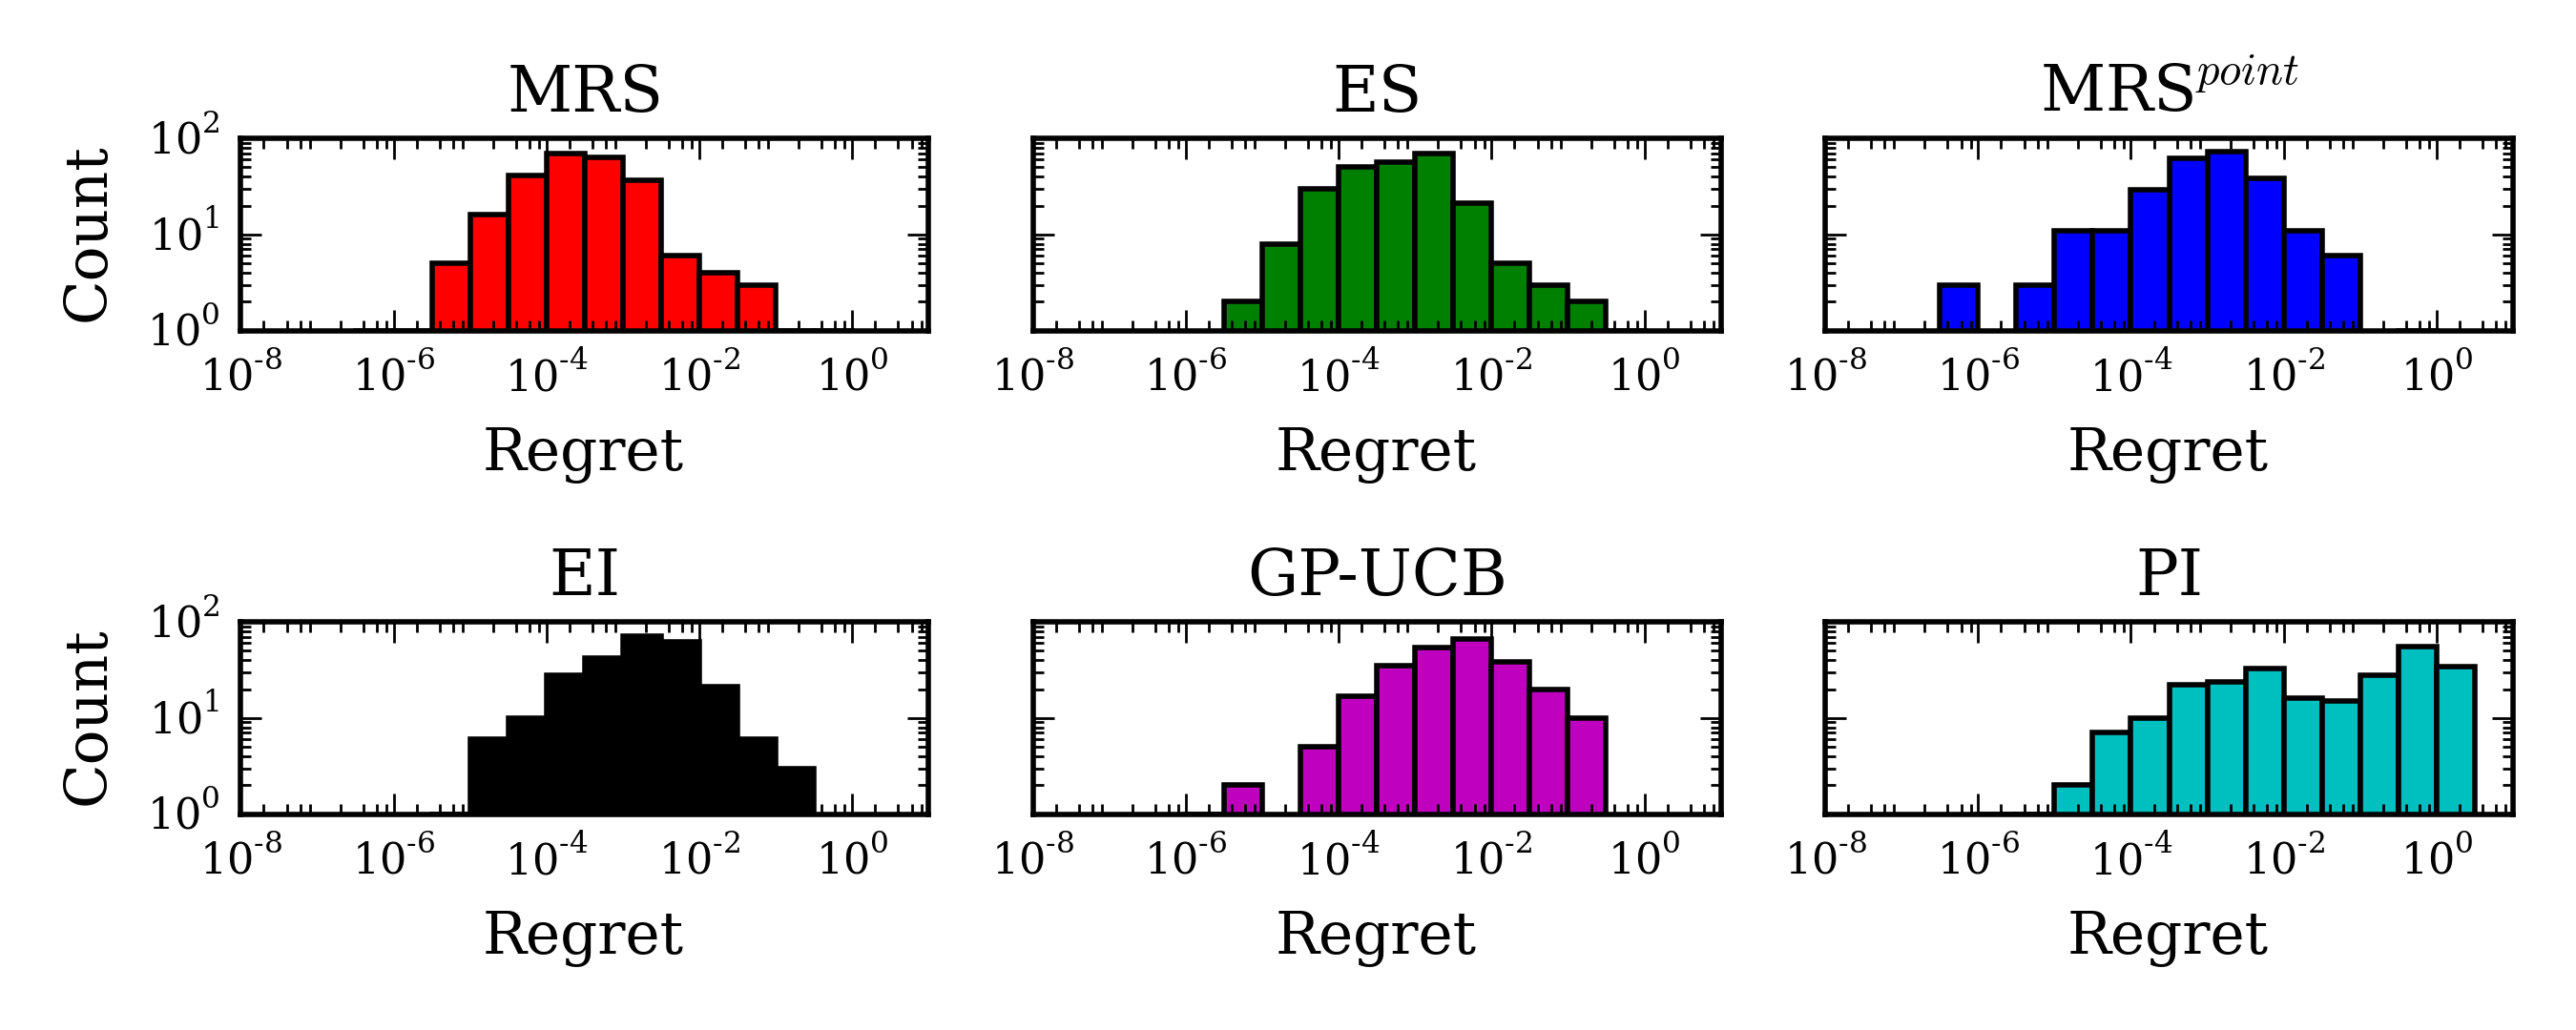
\includegraphics[width=.8\textwidth]{../pics/hist_mm}
\caption{Result for setting with \emph{model mismatch}}
\label{fig:empirical_comparison_mm}
\end{figure}

\end{center}
\end{block}

\begin{block}{\blocktitle{Outlook}}
\begin{itemize}
 \item For multi-task MRS and results on simulated robotic task: see paper
 \item Open questions: treatment of GP hyperparameters, more efficient approximation techniques for MRS, regret bounds for MRS?
 \item Source code: \url{https://github.com/jmetzen/bayesian_optimization}
\end{itemize}
\end{block}

\begin{block}{\blocktitle{References}}
\vspace*{-.75cm}
\begin{multicols}{2}
{\scriptsize
\setbeamertemplate{bibliography item}[text]
\bibliographystyle{abbrv}
\bibliography{../literature}
}
\end{multicols}

\end{block}
